%=========================================
% 	   Einleitung     		 =
%=========================================

\chapter{RSC Versuch}
\section{Einleitung}
Router und Switche begleiten uns im t�glichen Leben. Auch wenn sie oft nicht wahrgenommen werden, sind sie doch allgegenw�rtig. Ob mobiles Surfen, das Surfen am Computer oder auch telefonieren, diese T�tigkeiten sind ohne Router und Switche nicht m�glich. Der Netzwerkausr�ster Cisco Systems rechnet bis zu Jahr 2018 mit einem weltweiten Internettraffic von 1,6 Zettabyte \cite{cisco_traffic_schaetzung}. Die Netzwerke, die diesen Traffic behandeln und abwickeln sollen wachsen stetig mit ihren Aufgaben. Deswegen ist eine fundierte Ausbildung in der Netzwerktechnik und ein Verst�ndnis der Komponenten f�r den Informatiker der Zukunft unausweichlich. \todo{Kann man das so schreiben?}

Der folgende Versuch soll einen grundlegenden Einblick in den Aufbau eines Netzwerkes und die Konfiguration der Komponenten vermitteln.

\subsection{Ben�tigte Hardware f�r den Versuch}
F�r den Versuch werden ein Cisco 2811 Router und ein Cisco 2960 Switch ben�tigt. Zus�tzlich werden ein Windows Computer mit einem Terminal Emulationsprogramm und diverse Kabel ben�tigt.

\subsubsection{Router}
Die Aufgabe eines Routers, manchmal auch als Layer 3 Switch bezeichnet, ist es, zwischen mehreren Netzwerken der ISO/OSI Referenzmodells Schicht 3 zu vermitteln. Dazu besitzt ein Router mehrere (virtuelle) Ports, an denen die entsprechenden Netzwerke angeschlossen sind. Der Router, der f�r unseren Versuch zur Verf�gung stand ist vom Netzwerkausr�ster Cisco Systems und ist aus der Modellreihe 2811.

\begin{figure}[htbp] 
  \centering
     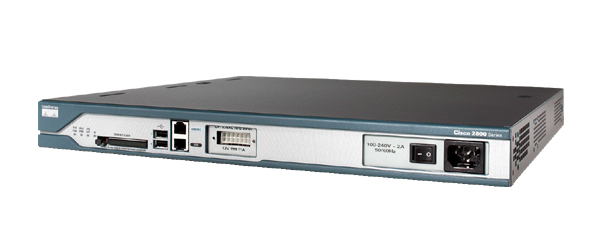
\includegraphics[width=0.6\textwidth]{tkinhalt/rsp_bilder/router.jpg}
  \caption{Ein Cisco 2800 Router \cite{cisco_2800_router}}
  \label{fig:router}
\end{figure}

\subsubsection{Switch}
Die Aufgabe eines Switches ist es, Netzwerksegmente miteinander zu verbinden. Das bedeutet, dass mehrere Kabel physikalisch miteinander verbunden werden k�nnen und die Datenpakete von einem Kabel in ein anderes weitergeleitet werden k�nnen. Logisch gesehen, werden die Datenpakete nur an die Kabel oder Ports weitergeleitet, die die Empf�ngeradresse dieses Pakets haben. Im Versuch stand uns ein Switch aus der Serie 2960 vom Netzwerkausr�ster Cisco Systems zur Verf�gung.

 \begin{figure}[htbp] 
  \centering
     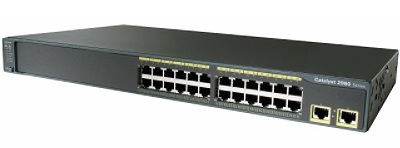
\includegraphics[width=0.6\textwidth]{tkinhalt/rsp_bilder/switch.jpg}
  \caption{Ein Cisco 2800 Router \cite{cisco_2960_switch}}
  \label{fig:switch}
\end{figure}

\subsubsection{Kabel}
